\section{Background}
\label{sec:background}

% yarim sayfa, turkce'ye ozel motivation
% en: locality, no morph
% tr: morph, free word order

\subsection{BoAT-v1}
\label{sec:boatvone}

% removing citation for anonymity ; ~\cite{turk-2021-boat}
% \boatvone~\cite{turk-2021-boat} is a standalone tool for annotating treebanks compatible with the \ud\ framework~\cite{ud}.
\boatvone~\cite{anon} is a standalone tool for annotating treebanks compatible with the \ud\ framework~\cite{ud}.
Although it was specifically developed for annotating Turkish treebanks, it supports agglutinative languages with rich morphologies; thus, it can be used for other languages as well.
It allows annotating one treebank at a time.
Annotations are stored in a file in \conllu\ format.
The file is updated during the annotation process.
It uses a validation script developed by \ud\ to dynamically display errors to the annotator as they annotate.
% \boatvone\ was used to create the \bountreebank~\cite{ud-turkish-boun} -- a manually annotated Turkish dependency treebank comprising 9,761 sentences from 5 different domains: essays, national newspapers, instructional texts, popular culture articles, and biographical texts.
\boatvone\ was used to create a manually annotated Turkish dependency treebank comprising 9,761 sentences from 5 different domains: essays, national newspapers, instructional texts, popular culture articles, and biographical texts.
It was implemented using Python~\cite{python} and Qt~\cite{qt}.

% main features of v1
% For annotation of any sentence, the annotator is shown a table which has a token per row with its corresponding columns (\id, \form, \udlemma, \upos, \xpos, \feats, \head, \deprel, \deps, and \misc\ as detailed in~\cite{turk-2021-boat}).
For annotation of any sentence, the annotator is shown a table which has a token per row with its corresponding columns (\id, \form, \udlemma, \upos, \xpos, \feats, \head, \deprel, \deps, and \misc\ as detailed in~\cite{anon}).
The annotator manually enters values for each column of each token.
It supports the splitting and joining of lemmas which are particularly significant for agglutinative languages since their tokens are often comprised of multiple morphemes whose accurate annotations sometimes require adjusting lemma boundaries by splitting or merging.
Tokens that are split result in additional two rows whose lemmas are then manually adjusted by an annotator such that they become distinct parts of a token.
Figure~\ref{fig:anno-fig-v1} shows annotation of a sentence.
The token ``yoktu'' (ID: 4-5) is split into ``yok'' (ID: 4) and ``tu'' (ID: 5).
Furthermore, it parses the \feats\ column's value into individual morphological features.

\begin{figure}[th!]
    \centering
        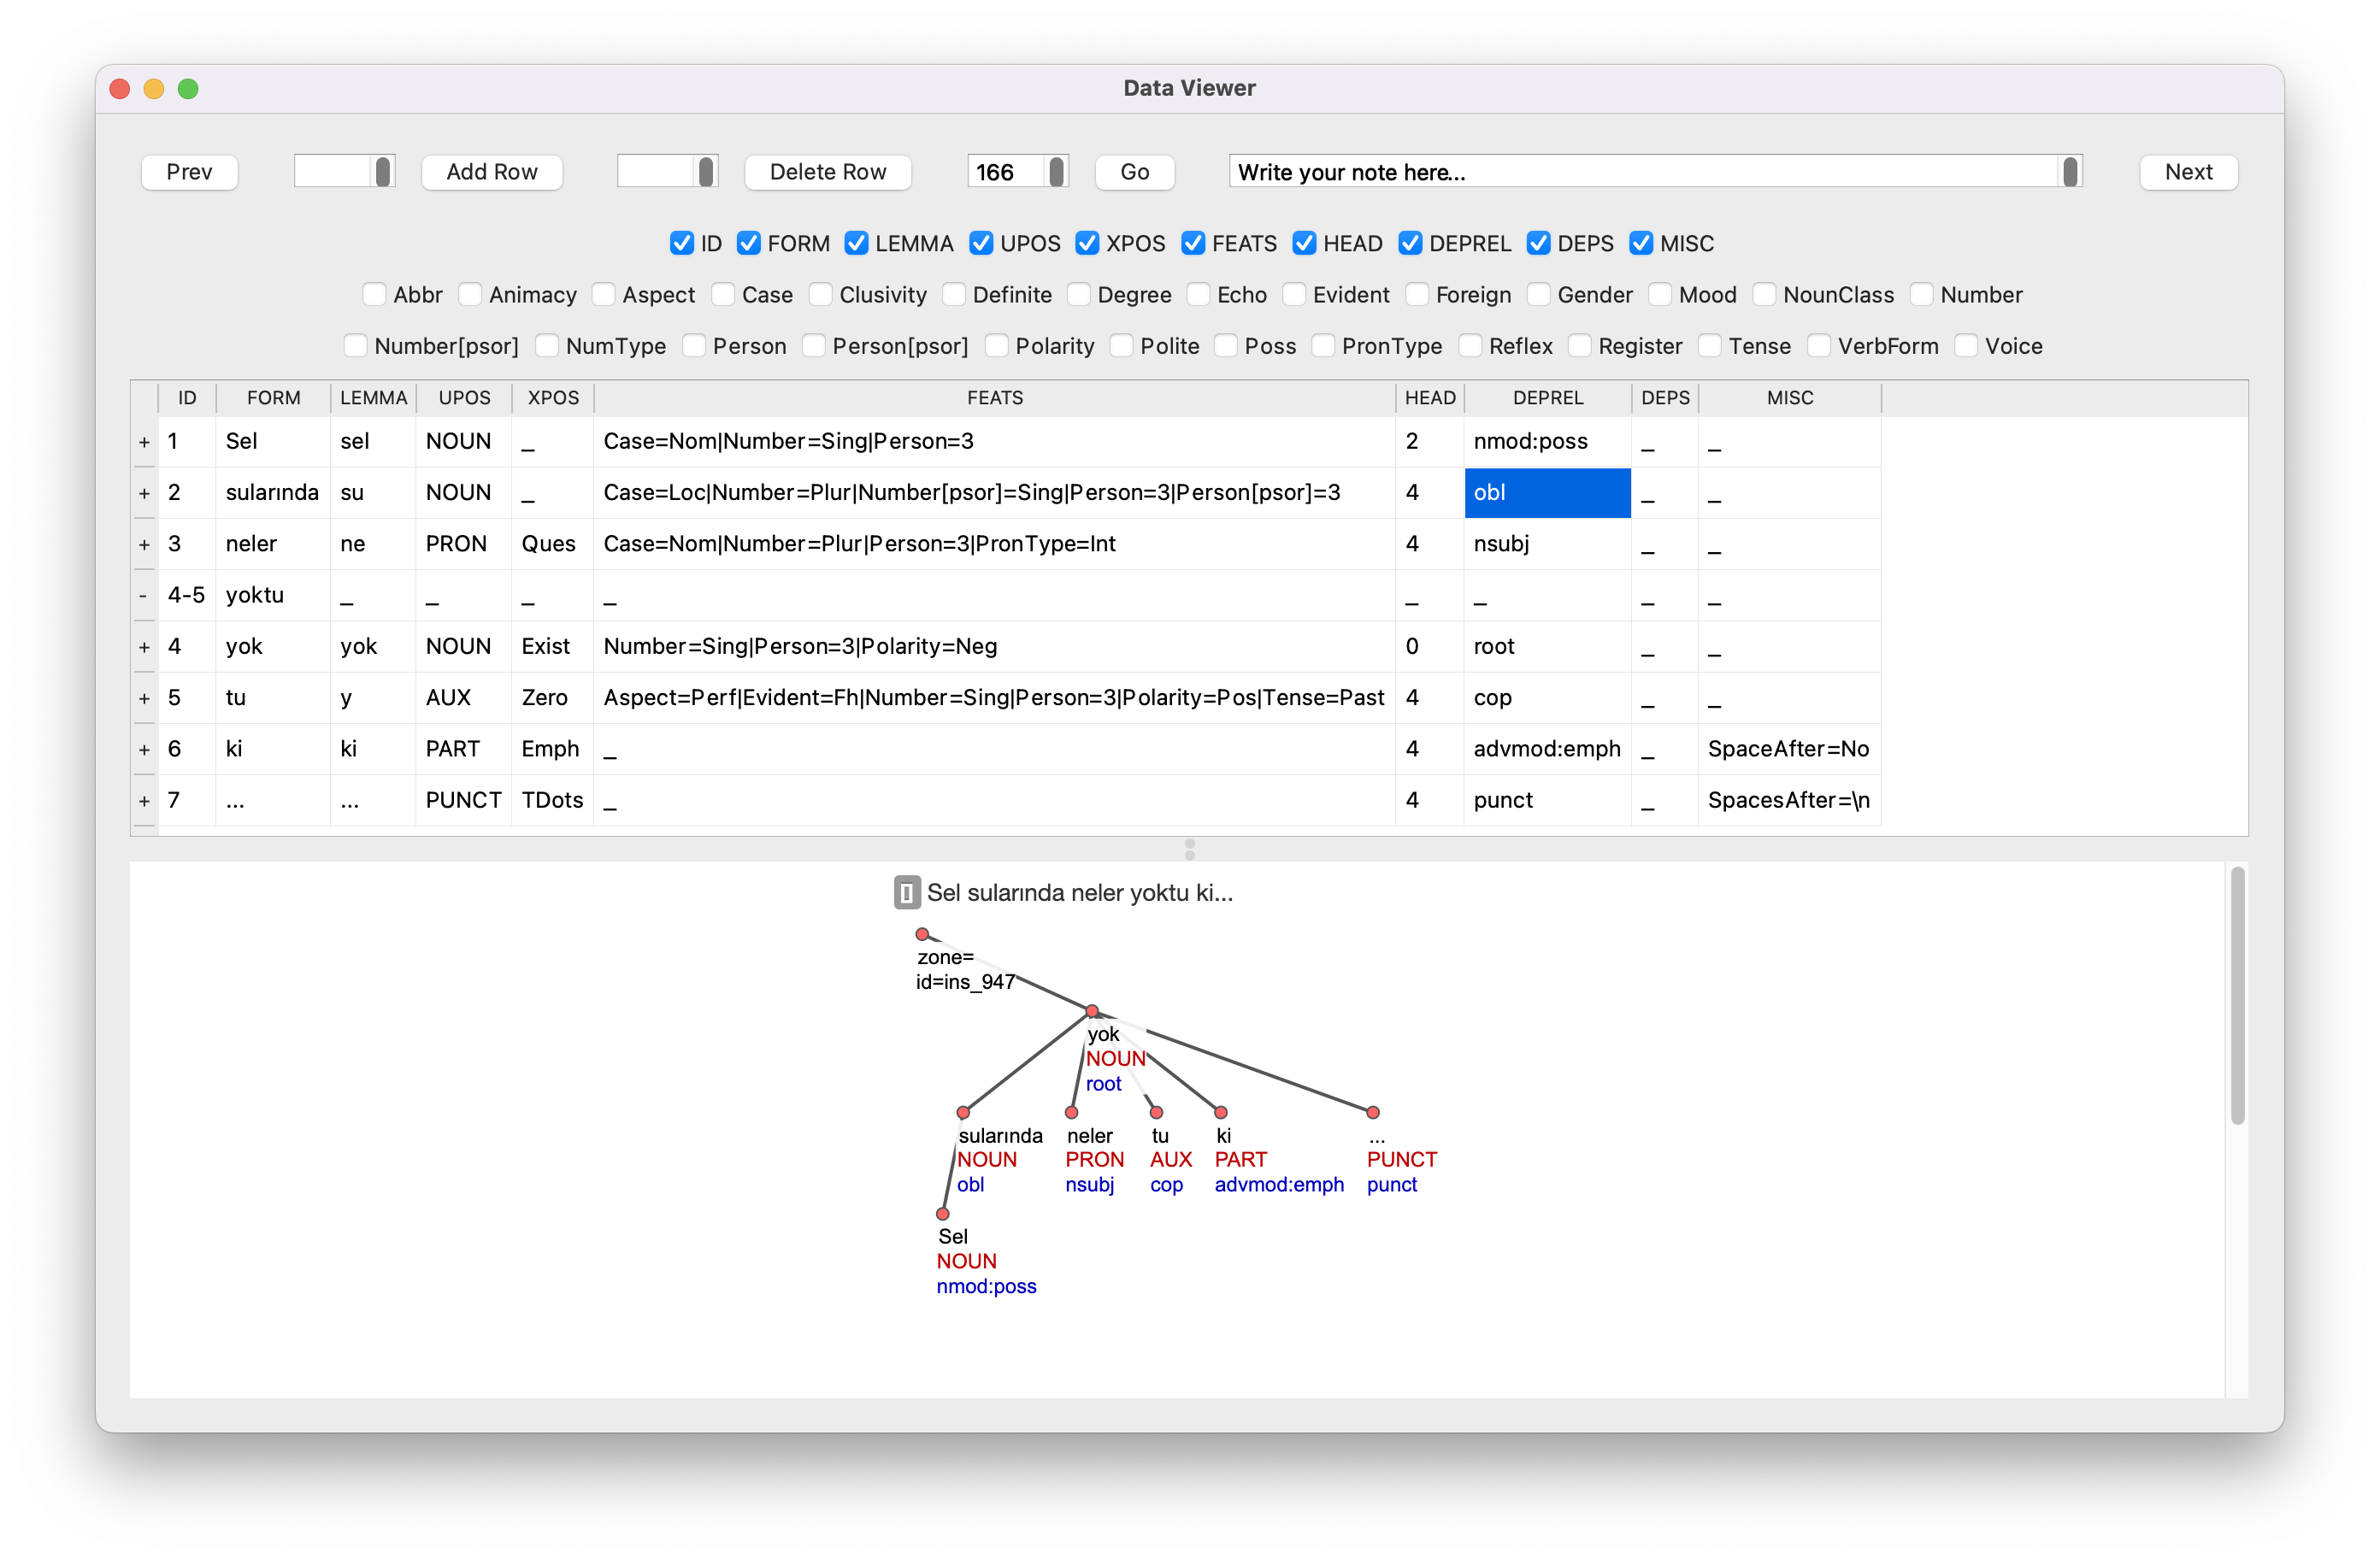
\includegraphics[width=0.8\textwidth]{figures/boat-v1-march-sample-annotation-mac.png}
        \caption{The annotation screen on \boatvone, captured while the sentence ``Sel sularında neler yoktu ki...'' is being annotated.}
        \label{fig:anno-fig-v1}
\end{figure}

\boatvone\ supports viewing features and their values individually under their corresponding columns (e.g. Case=Nom|Number=Sing|Person=3 can be shown in columns ``Case'', ``Number'', and ``Person'' with the values ``Nom'', ``Sing'', and ``3'').
It also allows the annotators to be able to take notes for specific annotations.

\subsection{Challenges of Agglutinative Languages}
\label{sec:challenges}
Agglutinative languages allow stacking multiple morphemes on a single root or stem to convey a wide range of linguistic information such as tense, aspect, number, person, possessor, and more.
Analytic languages, on the other hand, convey the same information through often free-standing function words.

A clear illustration of this contrast can be observed in \hyperref[trex]{Sentence (1)}: Each lemma of the Turkish sentence stacks at least two inflectional or derivational morphemes that carry out the function of free-standing morphemes in the corresponding English sentence.
Hence Turkish sentence has only 3 lemmas \textit{(masadaki, kitaplarını, görmüştüm)} while its English translation has 10 lemmas \textit{(I, had, seen, your, books, that, were, on, the, table)}.

\ex.
\label{trex}
Masa-da-ki \hspace*{.573cm}kitap-lar-ın-ı \hspace*{1.8cm}gör-müş-tü-m.\\
table-{\sc \Loc-\Der} book-{\sc \Pl-\Poss.\Second\Sg-\Acc} see-{\sc \Ant-\Pst-\First\Sg}\footnote{\printglossaries}\\
\textit{`I had seen your books that were on the table.'}

As a result of this contrast, lemmas in agglutinative languages like Turkish bear more features in the \feats\ column compared to isolating or analytic languages like English.
In addition to a higher feature-per-token count, agglutinative languages often have higher non-unique feature counts as well due to their rich repository of derivational and inflectional morphemes.

In order to offer an empirical example of this contrast, we compared non-unique features, total tokens, and features-per-token counts of multilingual \ud\ treebanks (ATIS and PUD)~\cite{atis-tr, atis-en, pud-tr, pud-en}.
Despite following different annotation customs, both Turkish treebanks have significantly higher non-unique features and lower token counts than their English counterparts (see \hyperref[table:feat-comp]{Table 1}).
As a result, both Turkish treebanks have more features per token, in fact, ATIS Turkish treebank has more than two times more features per token than ATIS English.

\newcolumntype{s}{>{\columncolor[HTML]{FFFAF0}} p{2.8cm}}
\begin{table}[h]
    \label{table:feat-comp}
    \centering
    \begin{tabular}{|s|>{\centering\arraybackslash} p{3.5cm}|>{\centering\arraybackslash} p{3cm}|>{\centering\arraybackslash} p{3cm}|}
       \hline
        \rowcolor[HTML]{FFFAF0} \multicolumn{4}{|c|}{\textbf{Comparison of \ud\ Treebanks}} \\ \hline\hline
        \multicolumn{1}{|c|}{\cellcolor[HTML]{FFFAF0} \textbf{Treebank}} & \textbf{Non-unique feats} & \textbf{Total tokens} & \textbf{Feats per token} \\\hline
        ATIS Turkish & 112,214 & 45,875 & 2.45 \\\hline
        ATIS English & 63,434 & 61,879 & 1.03 \\\hline
        PUD Turkish & 32,583 & 16,536 & 1.97 \\\hline
        PUD English & 23,995 & 21,176 & 1.13 \\\hline
    \end{tabular}
    \caption{Comparison of morphological feature annotations of Turkish and English \ud\ treebanks with equivalent sets of sentences in terms of meaning.}
\end{table}

In addition to having a higher feature count, being a free word order language makes annotating Turkish treebanks substantially challenging.
As Turkish allows scrambling and topicalization, the average dependency length per token in Turkish sentences is much higher than in fixed word order languages like English.
Moreover, such word order changing operations also affect headedness and the dependency arc direction while changing dependency lengths: The order of a dependent and its head can vary within or across the sentences (compare \hyperref[dep1]{Sentence 1} and \hyperref[dep2]{Sentence 2}).

\begin{multicols}{2}
\vspace*{\fill} 
\ex. \label{dep1}
\begin{dependency}
   \begin{deptext}
      Siyah \& kediyi \& ben \& gördüm \& sokakta \& . \\
   \end{deptext}
   \depedge{4}{3}{nsubj}
   \depedge{2}{1}{amod}
   \depedge{4}{2}{dobj}
   \depedge{4}{5}{obl}
   \depedge{4}{6}{punct}
\end{dependency} \\
Lit. The black cat I saw on the street. \\
\textit{‘I saw the black cat on the street.’} \\
\vspace{.05cm} \\
\textbf{Average arc length:} 1.4\\
\textbf{Longest arc length:} 3\\
\columnbreak

\ex. \label{dep2}
\begin{dependency}
   \begin{deptext}
      Gördüm \& sokakta \& siyah \& kediyi \& ben \& . \\
   \end{deptext}
   \depedge{1}{5}{nsubj}
   \depedge{1}{2}{obl}
   \depedge{4}{3}{amod}
   \depedge{1}{4}{dobj}
   \depedge{1}{6}{punct}
\end{dependency} \\
Lit. Saw on the street the black cat I. \\
\textit{‘I saw the black cat on the street.’} \\
\vspace{.05cm} \\
\textbf{Average arc length:} 2.8\\
\textbf{Longest arc length:} 5
%%% YOU NEED A NEW LINE BEFORE multicols -- SUZAN

\end{multicols}

As a result, an annotation interface designed for agglutinative languages must facilitate the annotator's job despite the changes in dependency length and arc direction.

As the dependency length increases, drag-drop interfaces become impractical since they require the annotator to drag lemmas for longer distances, thus decreasing the annotation speed and increasing the effort.
Moreover, the need to annotate more features per token also makes drag-drop interfaces very difficult to use for annotating agglutinative languages.
Thus, opting for an interface that utilizes the keyboard and allows typing is more practical for such languages.

In addition to the data entry method (the mouse vs the keyboard), feature-per-token counts, and changes in the dependency length and arc direction also require some adjustments in the interface.
For instance, the annotation interface must display the entire sentence and all lemma ids at all times.
This way, the annotator can see the head and/or dependent of the lemma that is being annotated even though they are dealing with a very verbose sentence or a very high dependency length.
Moreover, the annotation interface must be able to display large numbers of tags in the features column in an easy-to-read way so that the annotator can keep track of the annotation even when they are dealing with particularly packed lemmas.

% UD_English-ATIS/stats.xml:
% Non-unique feats: 63434
% Total tokens: 61879
% Feats per token: 1.0251296885857883

% UD_Turkish-ATIS/stats.xml:
% Non-unique feats: 112214
% Total tokens: 45875
% Feats per token: 2.4460817438692097

% UD_German-PUD/stats.xml:
% Non-unique feats: 56987
% Total tokens: 21000
% Feats per token: 2.7136666666666667

% UD_Turkish-PUD/stats.xml:
% Non-unique feats: 32583
% Total tokens: 16536
% Feats per token: 1.9704281567489115

% UD_Korean-PUD/stats.xml:
% Non-unique feats: 13430
% Total tokens: 16584
% Feats per token: 0.8098166907863

% UD_Spanish-PUD/stats.xml:
% Non-unique feats: 48819
% Total tokens: 22822
% Feats per token: 2.1391201472263606

% UD_Italian-PUD/stats.xml:
% Non-unique feats: 40715
% Total tokens: 22182
% Feats per token: 1.8354972500225408

% UD_French-PUD/stats.xml:
% Non-unique feats: 47560
% Total tokens: 24131
% Feats per token: 1.970908789523849

% UD_English-PUD/stats.xml:
% Non-unique feats: 23995
% Total tokens: 21176
% Feats per token: 1.1331224027200604

% explain comparison in table here
